\chapter{Hardware}

\begin{figure} [H]
    \centering
    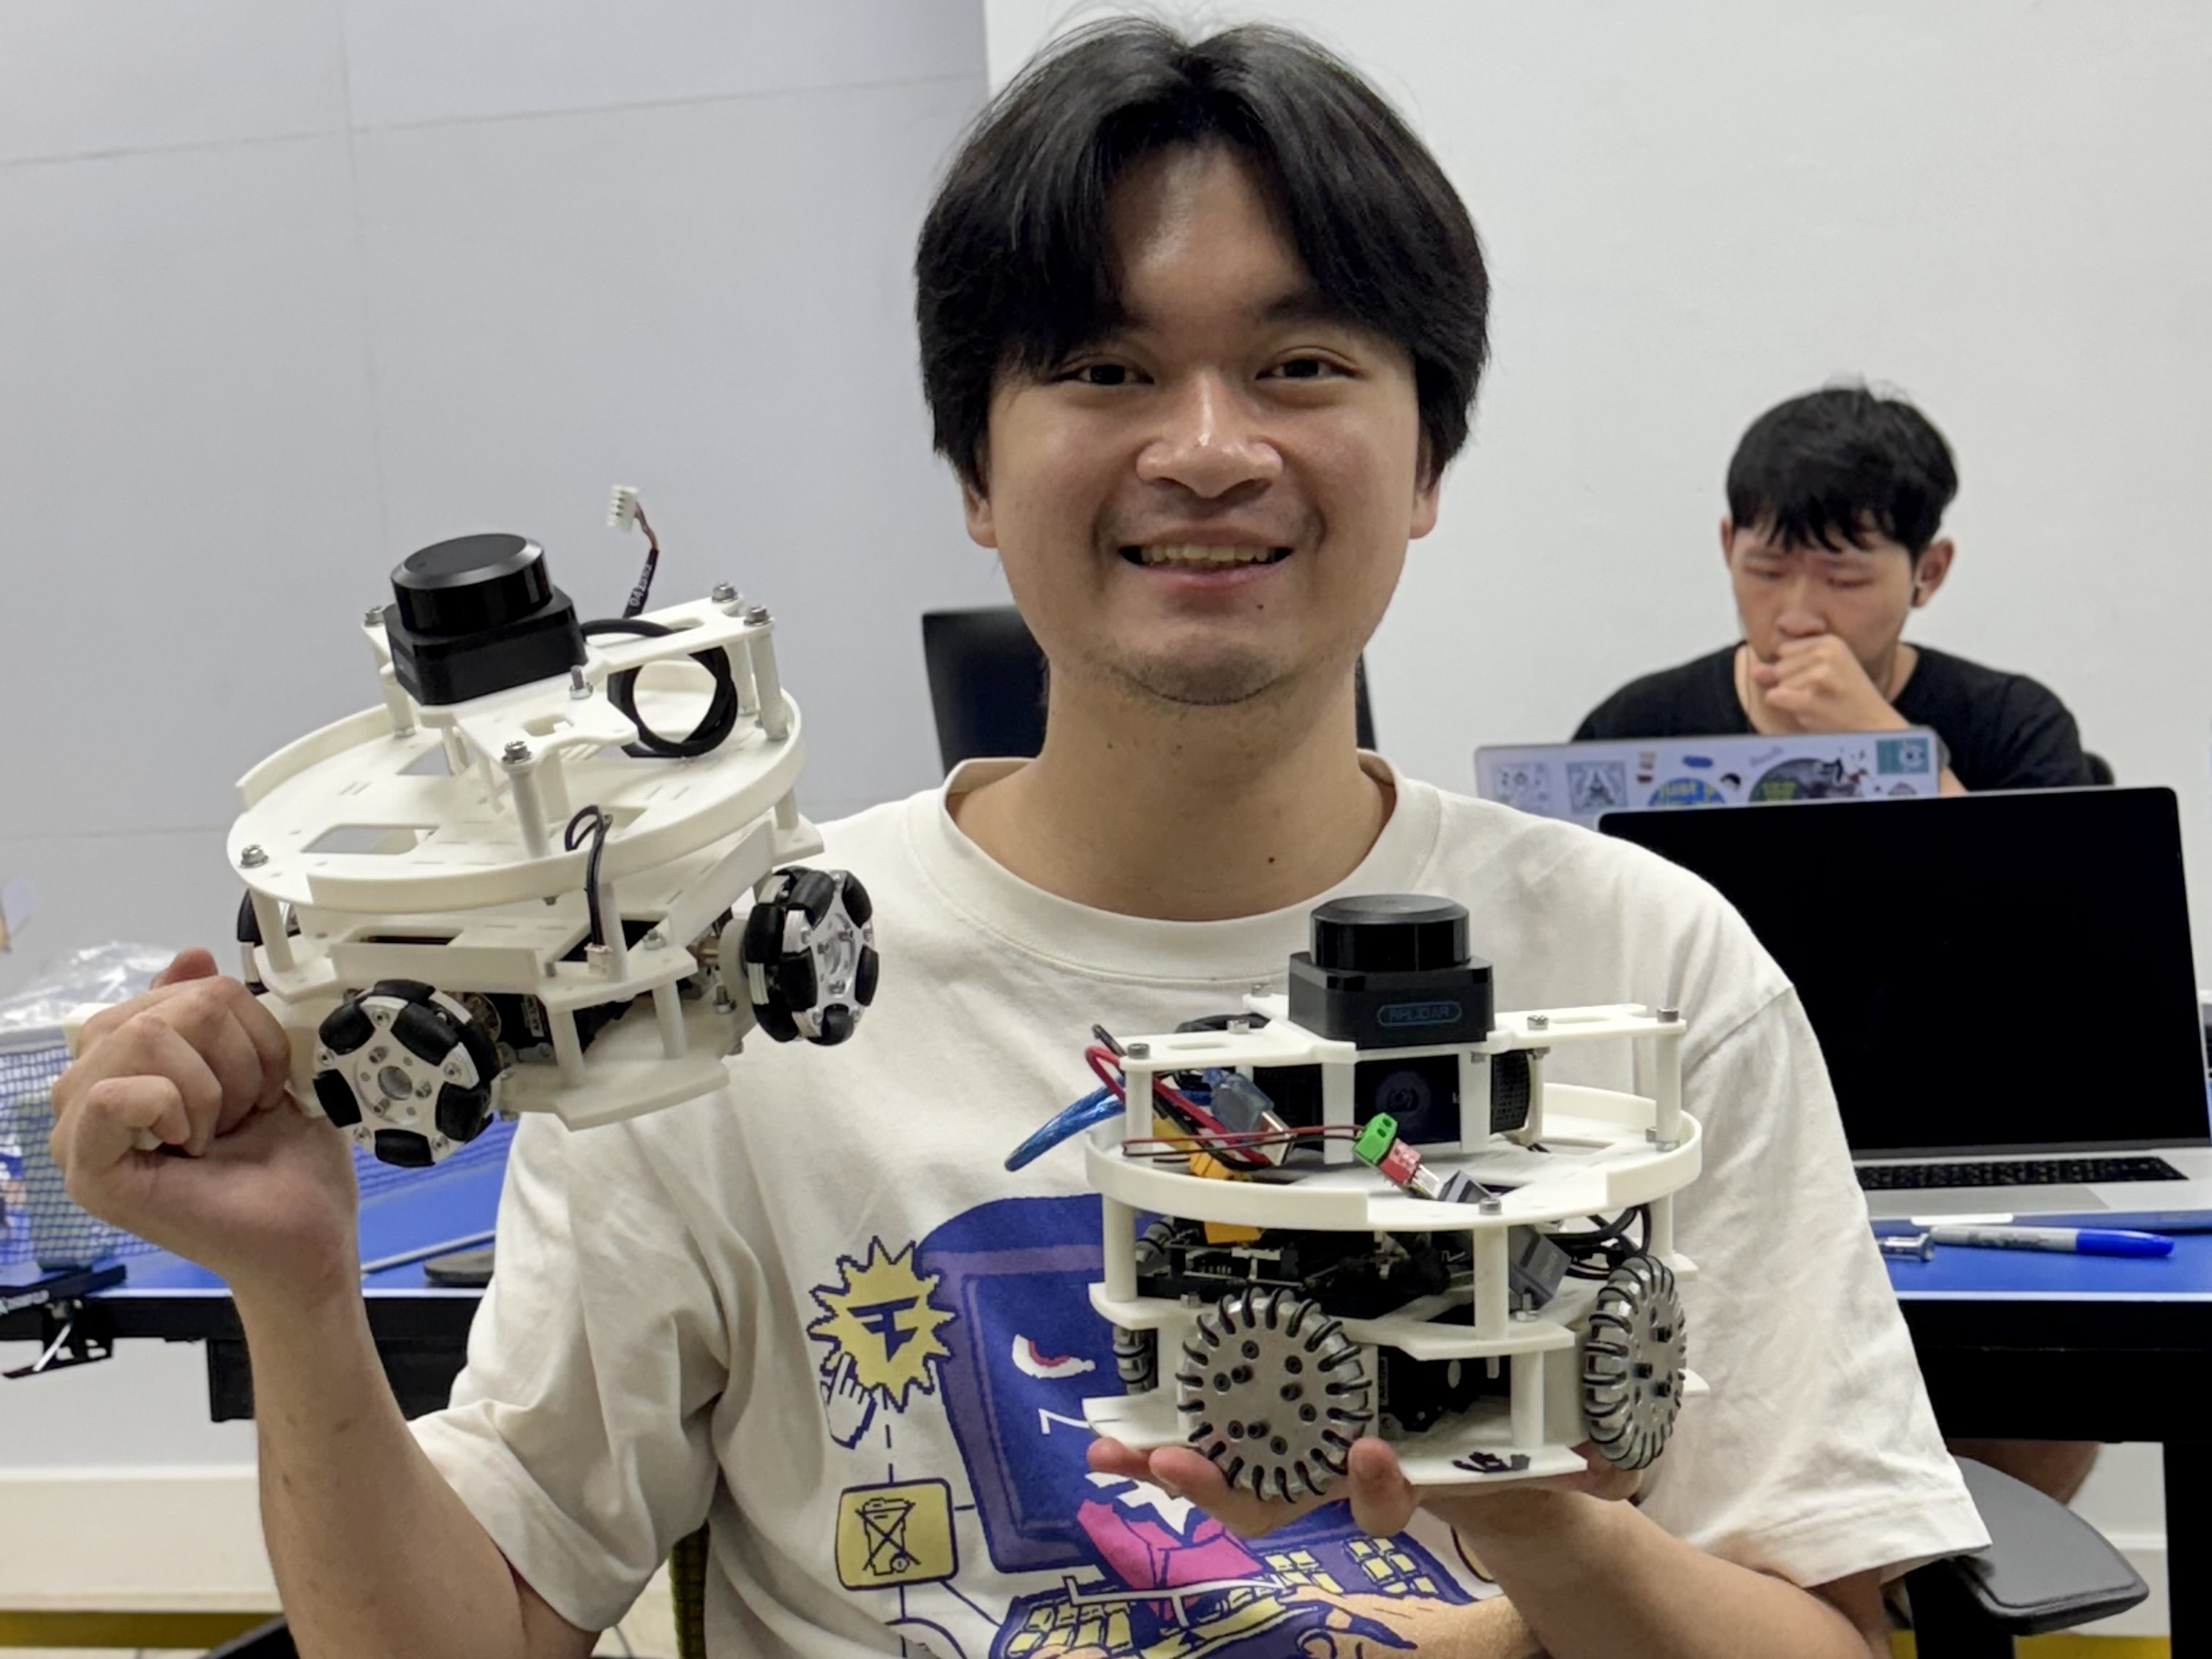
\includegraphics[width=0.65\linewidth]{assets/images/hardware/IMG_8290.jpeg}
    \caption{A happy man holding 2 built robots}
    \label{fig:have2robots}
\end{figure}
For hardware we have built the second robot with ease. Redesigning to incorporate metal parts were in order. The image on the left of the \ref{fig:hdinfo-1}(left), are 6 mm metal shaft to replace the PLA 3D printed ones. The middle image is the robot with the metal shafts attached the motor with a 6 mm flange coupler and the omni-wheel; A 6 mm journal bearing is used to off-load the shear stress to motor, it's pressed-fit into a 3D printed pillow block as we couldn't find a machined parts in-time. The right image is the robot with the metal shafts attached and the wheels attached. 
The omni-wheel are now newly bought from a local supplier with thicker rubber which helps to reduce slip, much improved from the first robot, which had a lot of slip. The robot is now able to move in all directions with ease. Further testing are required to imperially prove the improvement. Despite the base still made from 5 mm 3D printed PLA, it's quite rigid, we plan to change the plate to 5 mm acrylic to test the rigidity of the base. As according to a paper, 3D printed PLA has a range of Young's modulus of 2.1 to 4.4 GPa, while acrylic has a Young's modulus of 3.6 GPa. Therefore, hard to conclude with this better without proper testing. 

\begin{figure} [H]
    \centering
    \begin{tabular}{@{}c@{\hspace{0.5cm}}p{8cm}@{\hspace{0.5cm}}c@{}}
        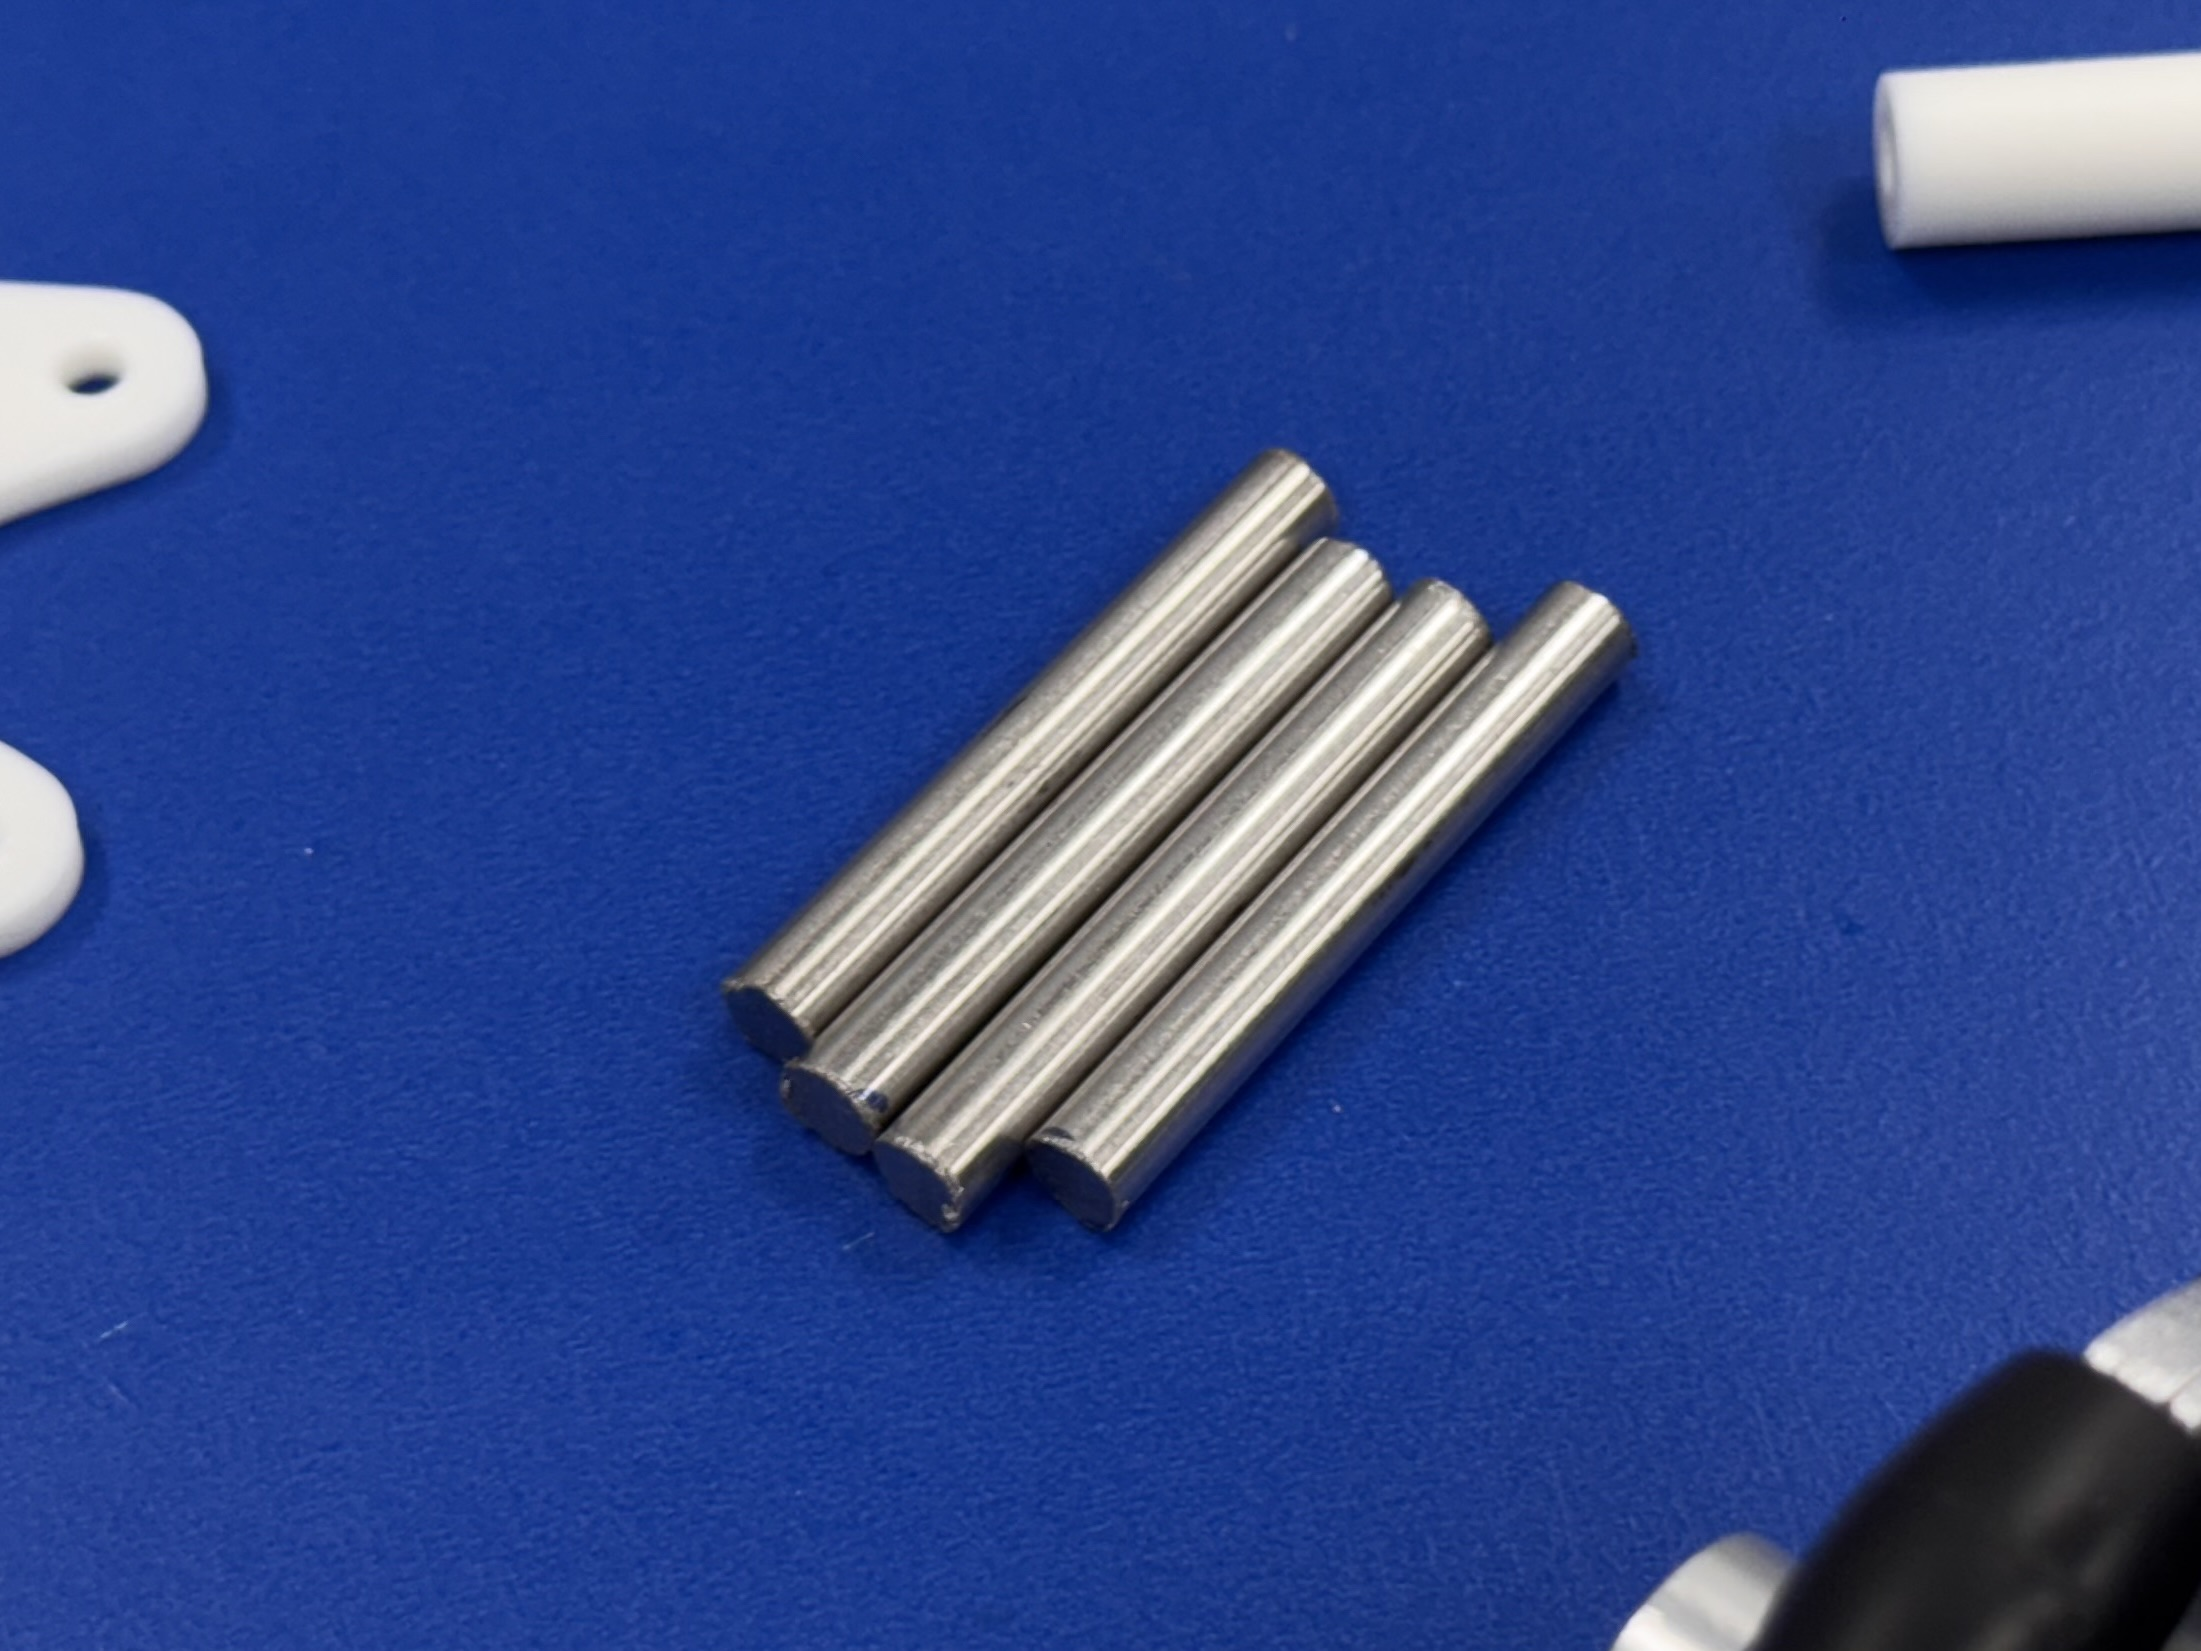
\includegraphics[width=0.5\textwidth]{assets/images/hardware/IMG_8280.jpeg} &
        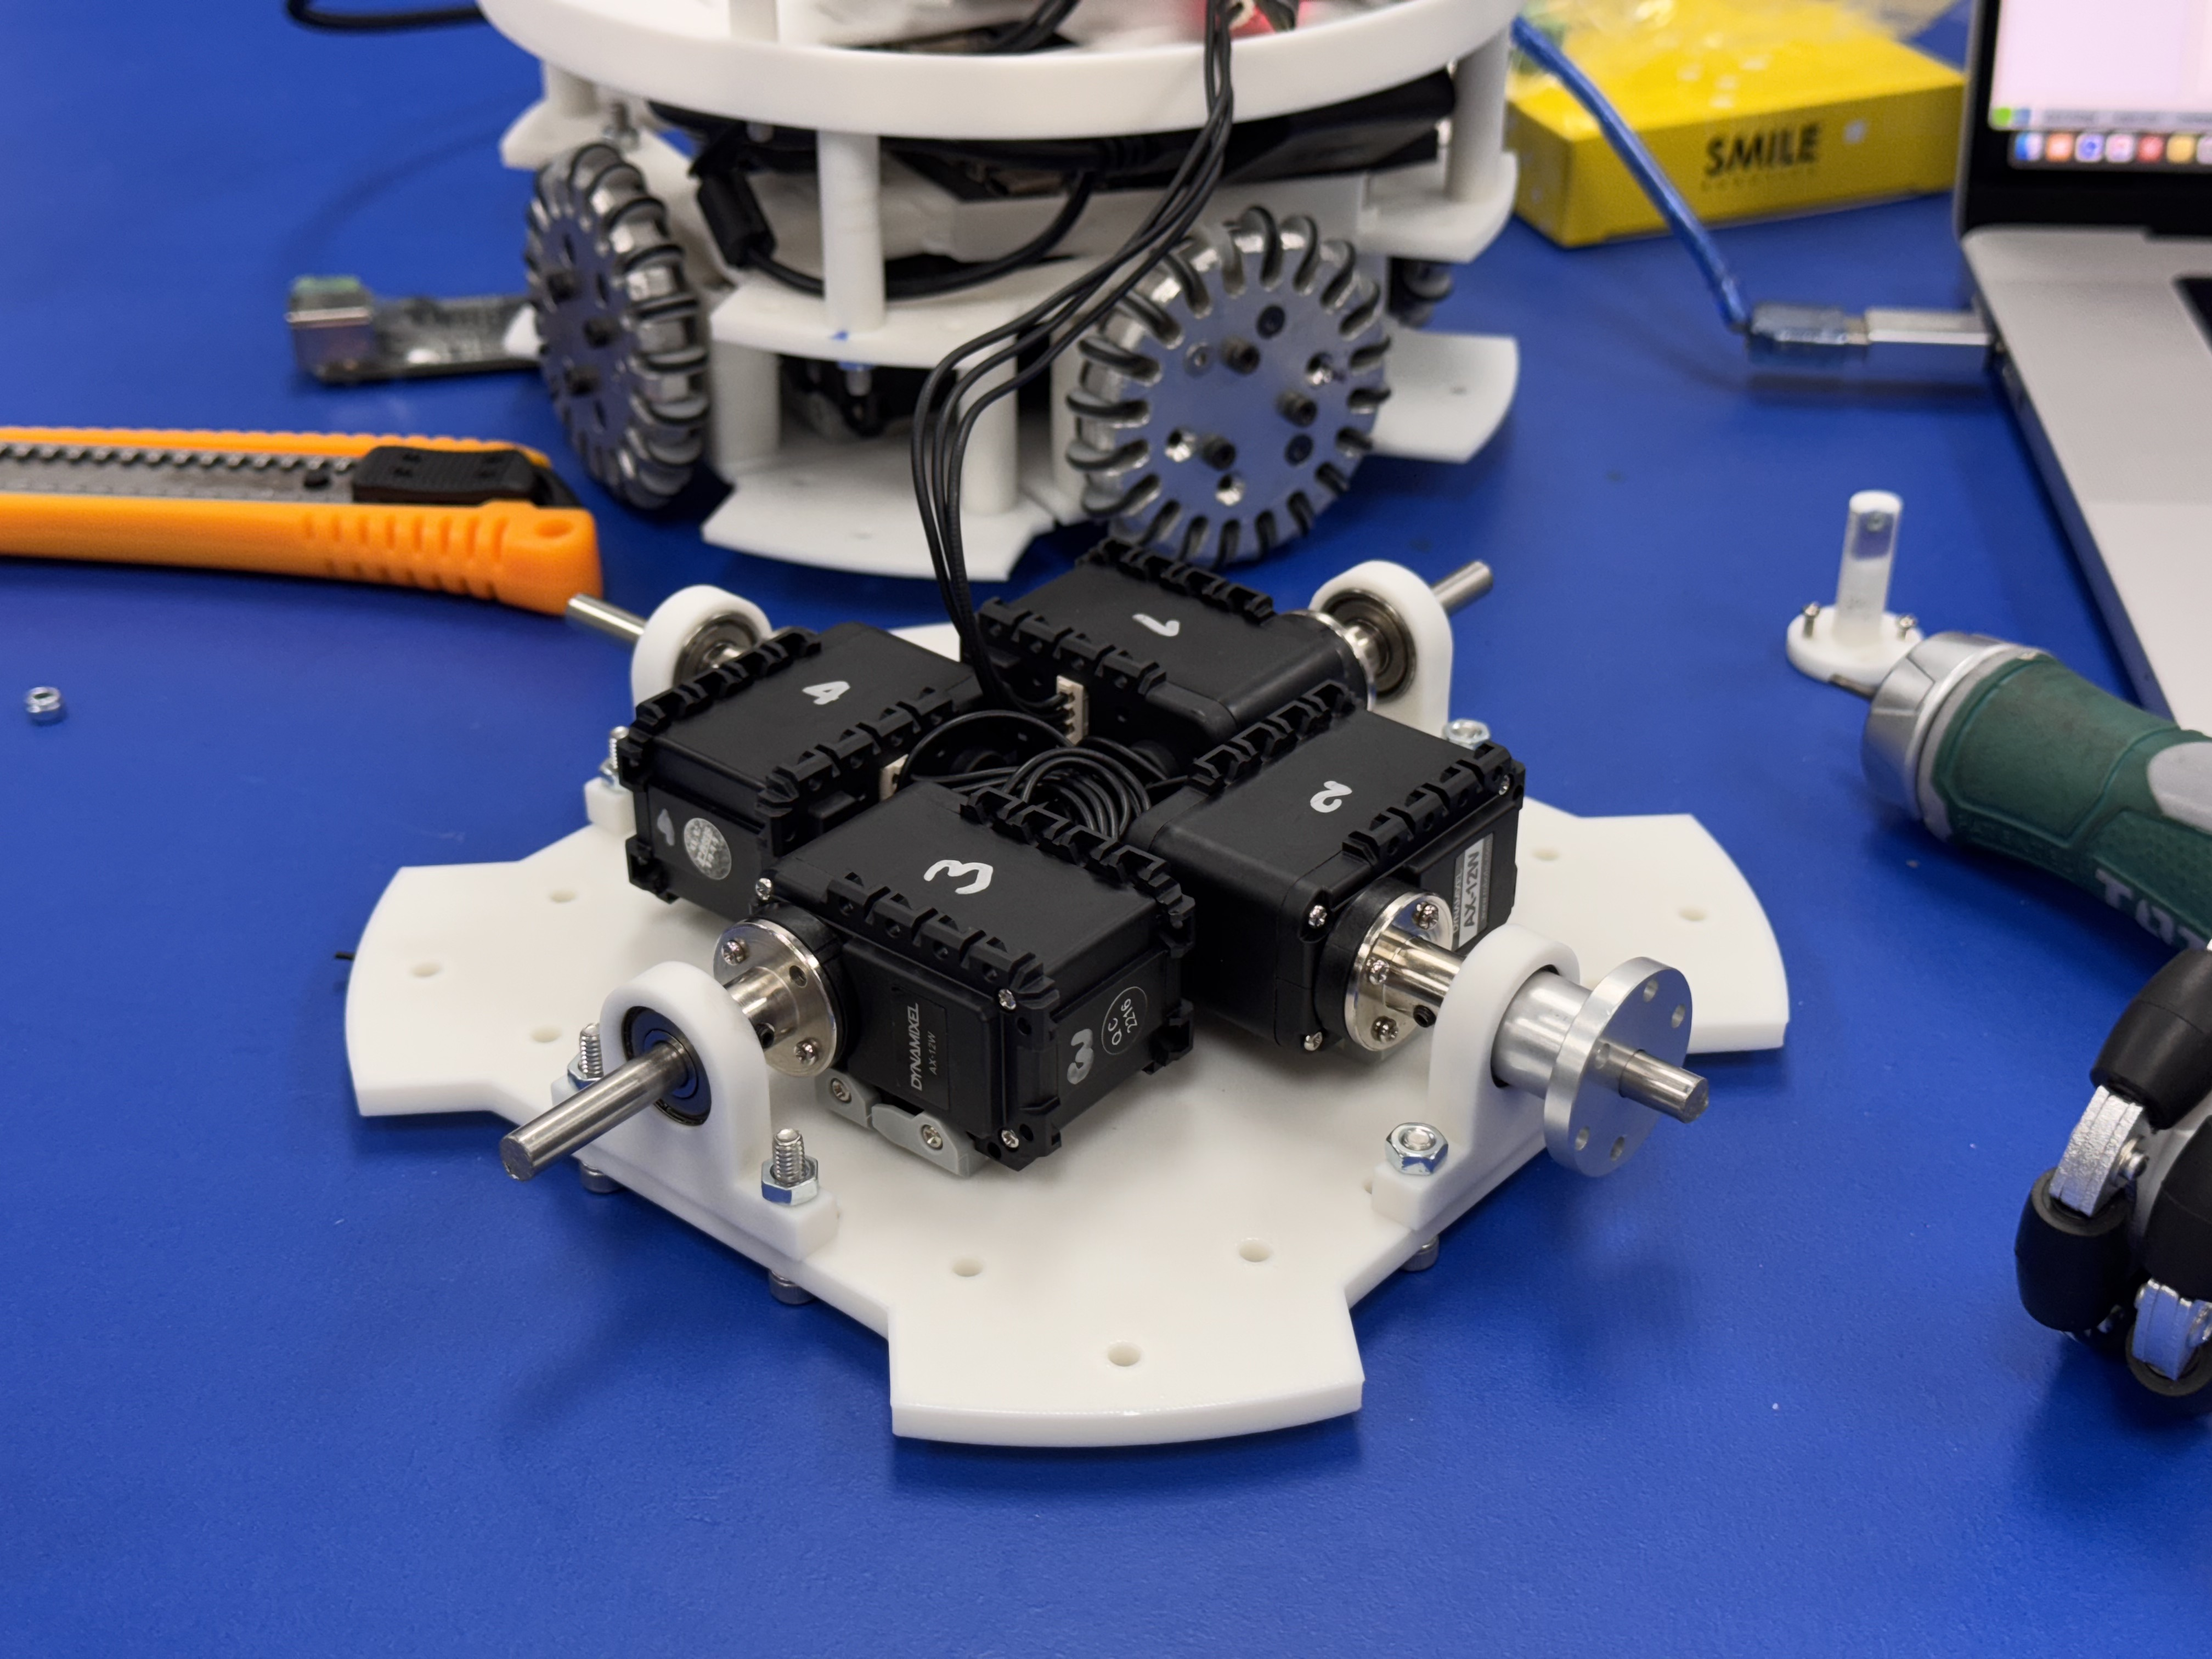
\includegraphics[width=0.5\textwidth]{assets/images/hardware/IMG_8284.jpeg} & \\
        \small Sliced Metal Shafts &
        \small Assembly of the motors, motor flange, bearing pillow block, omni-wheel flange&
    \end{tabular}
    \caption{}
    \label{fig:hdinfo-1}
\end{figure}
\begin{figure} [H]
    \centering
    \begin{tabular}{@{}c@{\hspace{0.5cm}}p{8cm}@{\hspace{0.5cm}}c@{}}
        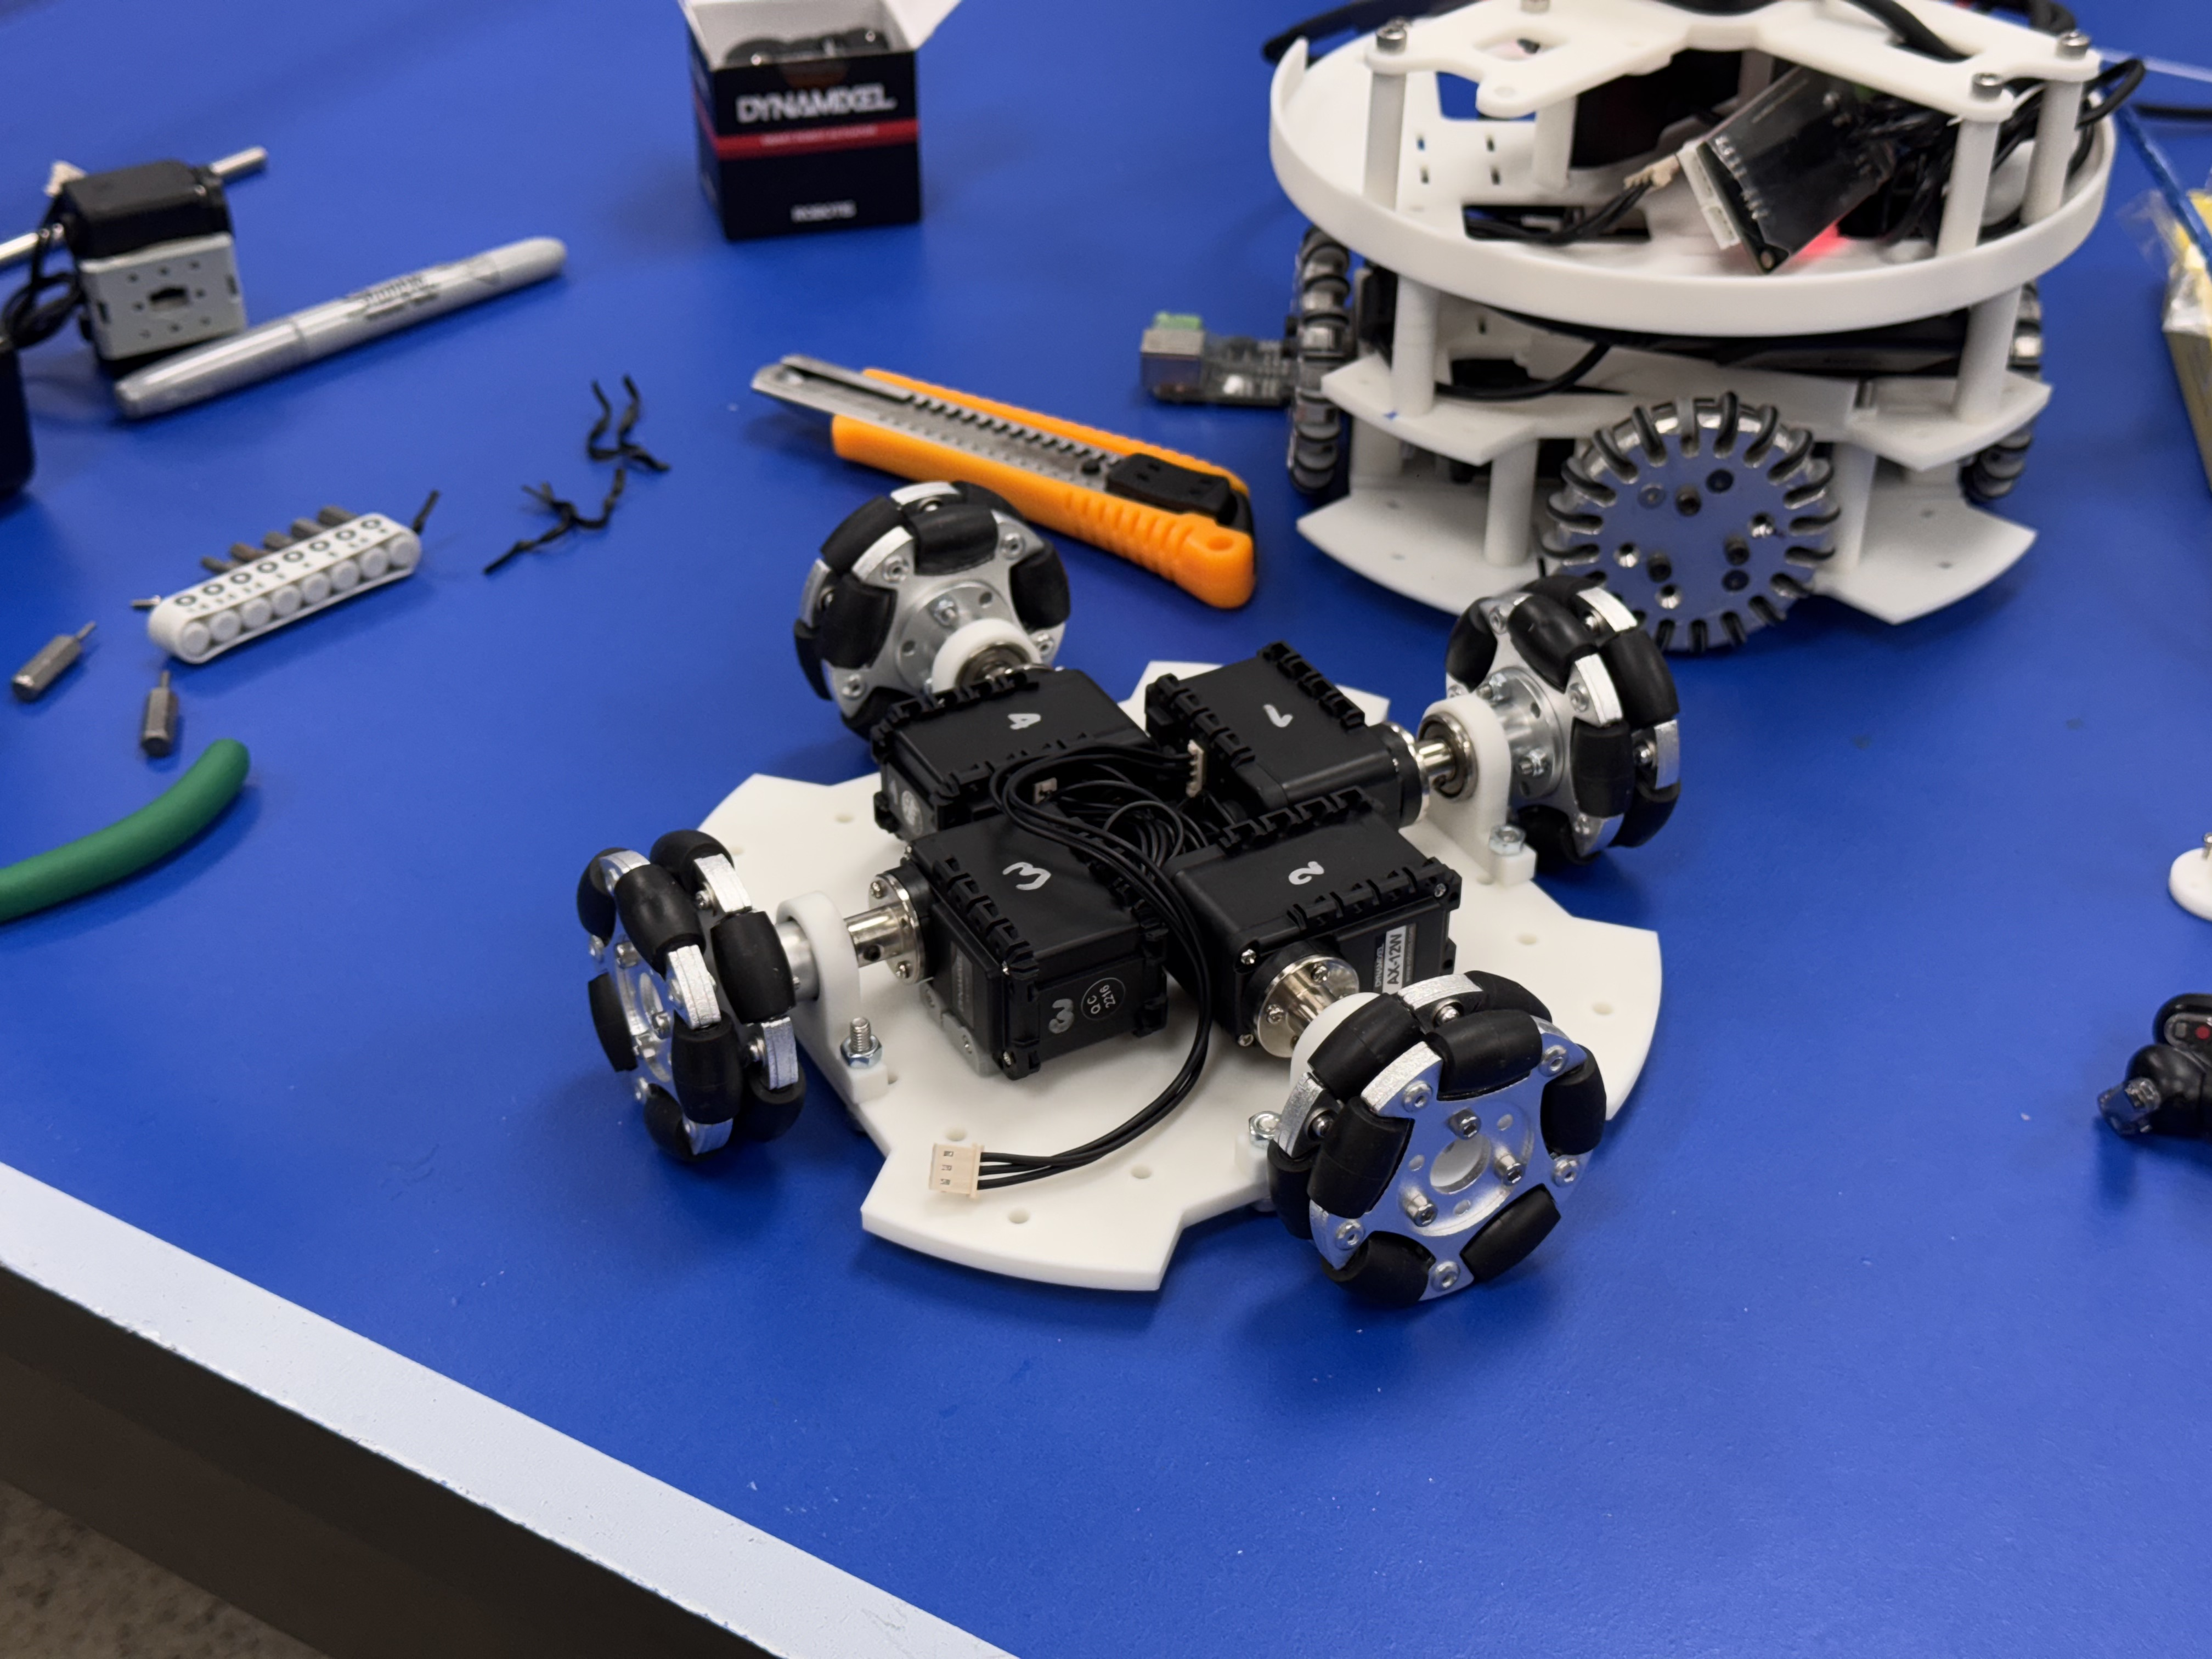
\includegraphics[width=0.5\textwidth]{assets/images/hardware/IMG_8286.jpeg} &
        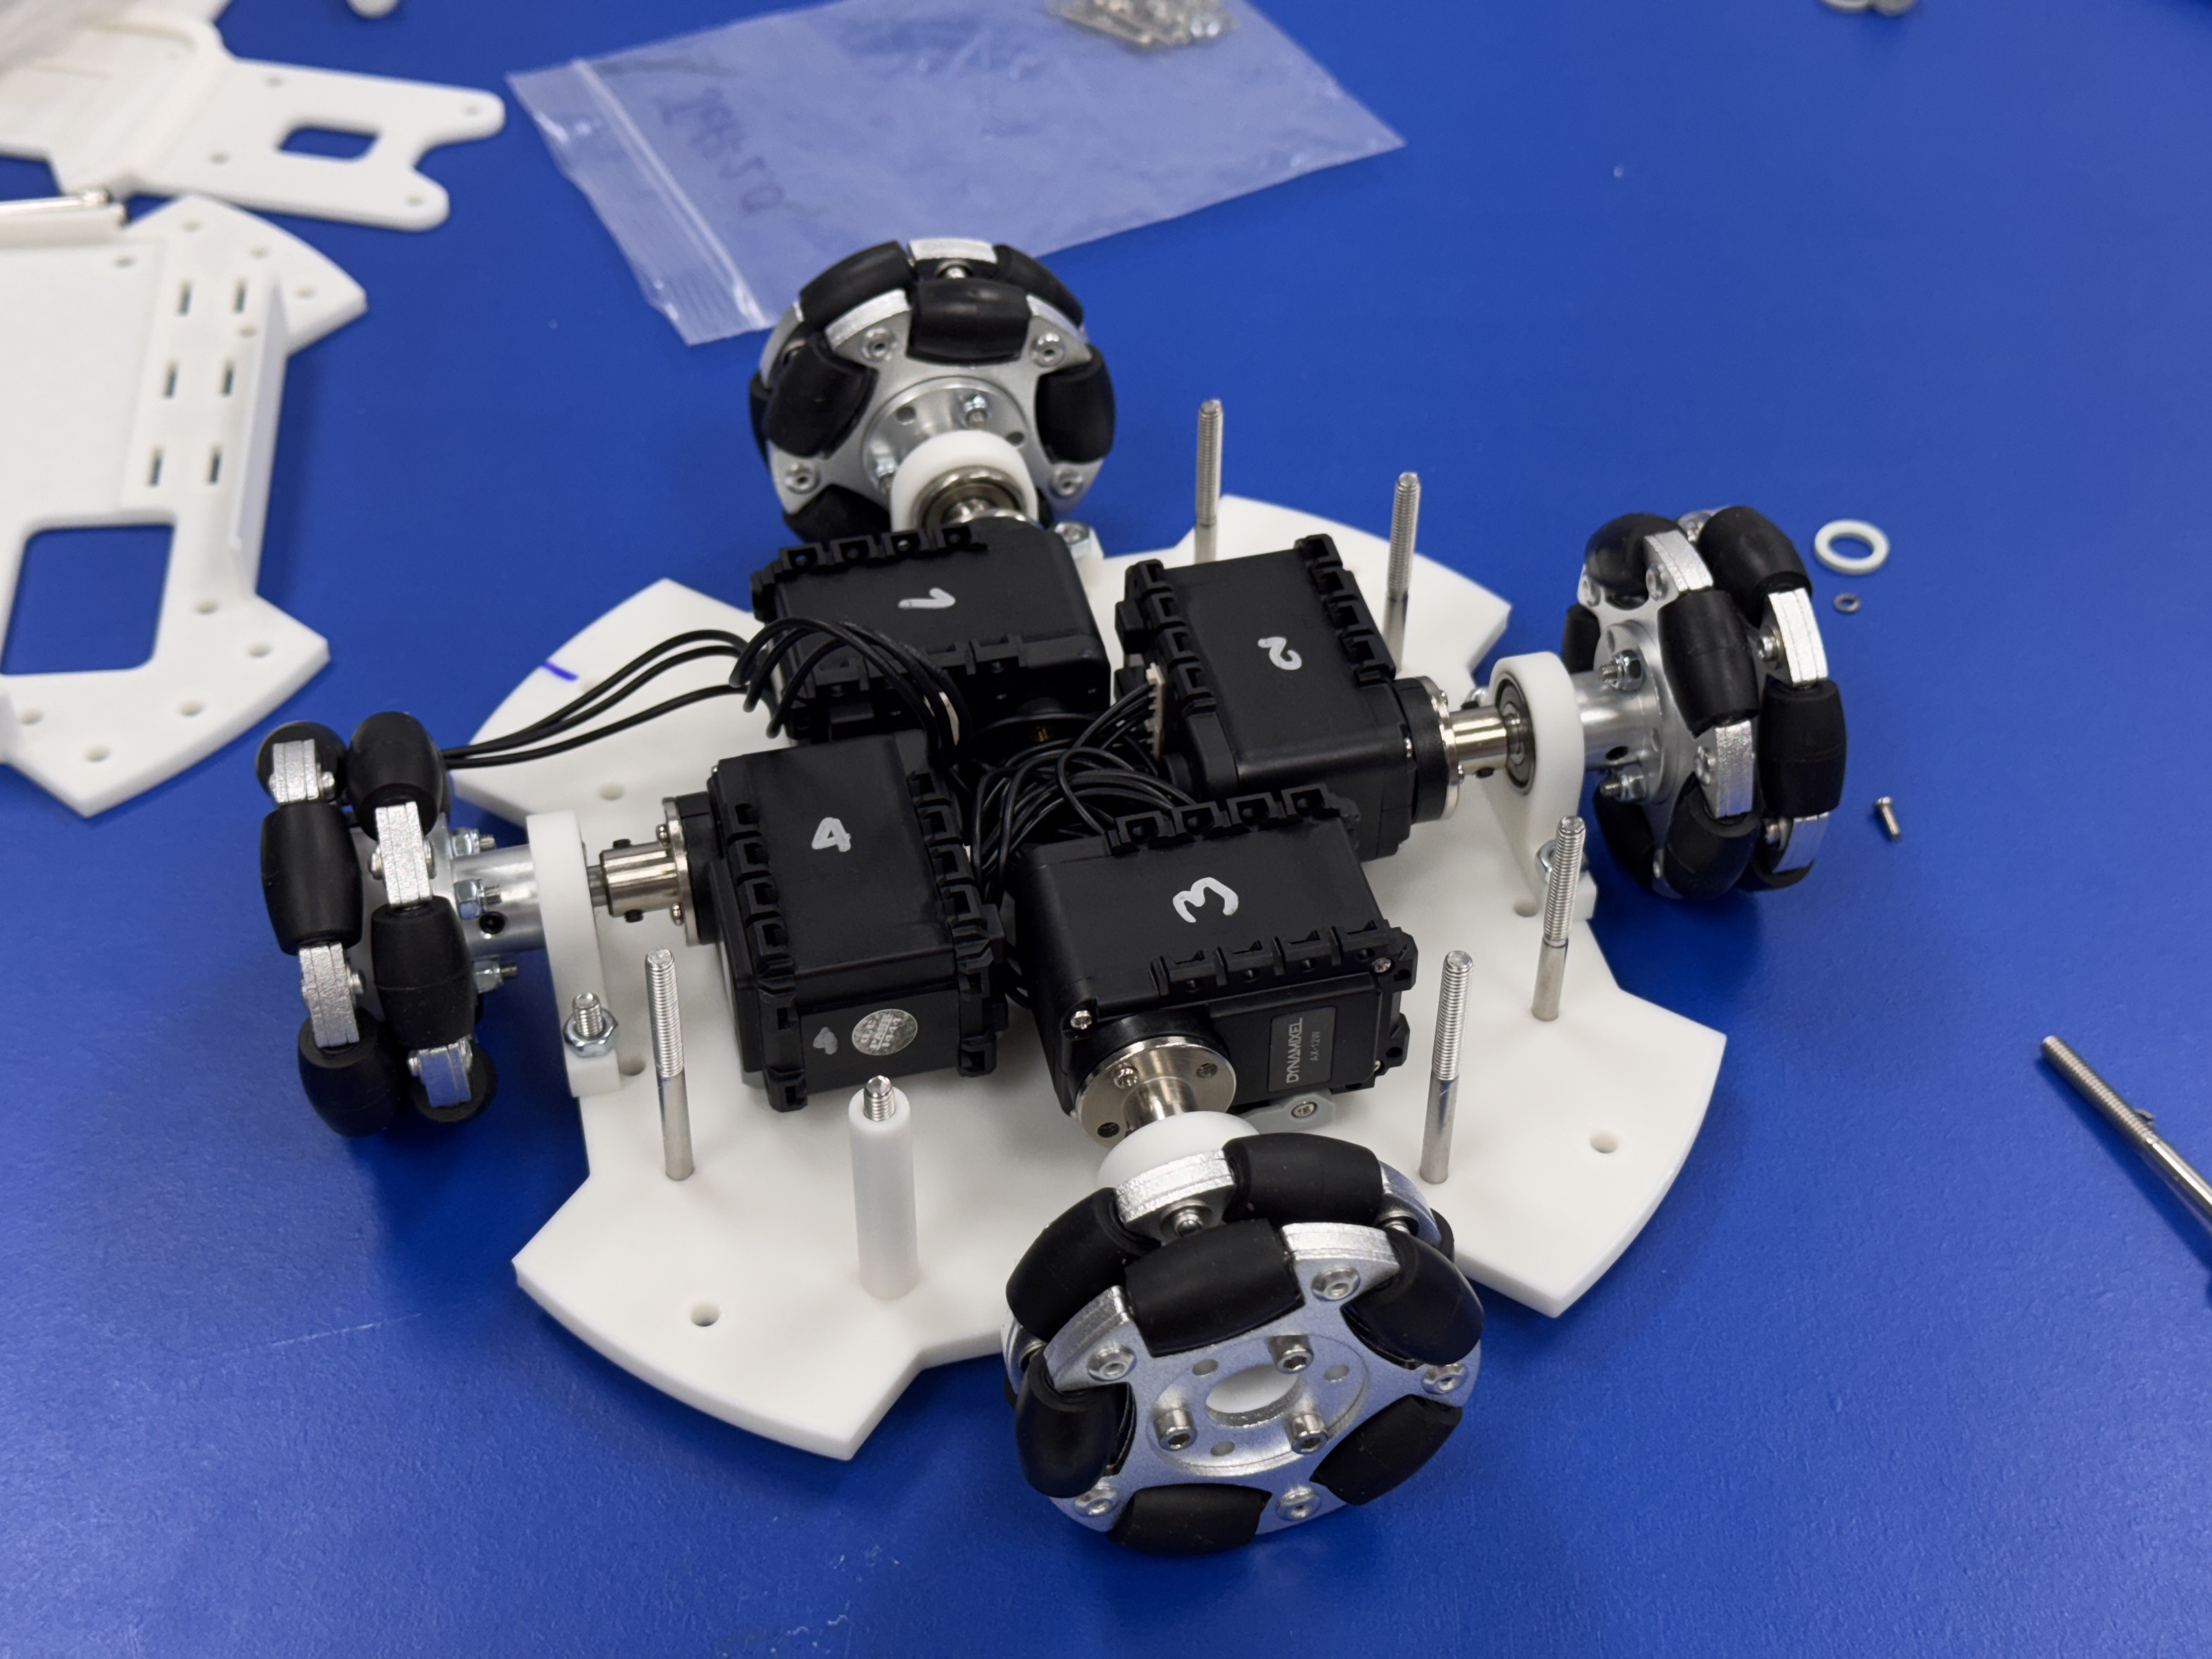
\includegraphics[width=0.5\textwidth]{assets/images/hardware/IMG_8287.jpeg} & \\
        \small Assembly of \ref{fig:hdinfo-1}(right) with omni-wheel attached  &
        \small Assembly of \ref{fig:hdinfo-1}(right) with omni-wheel attached + standoffs + screws &
    \end{tabular}
    \caption{}
    \label{fig:hdinfo-2}
\end{figure}
% 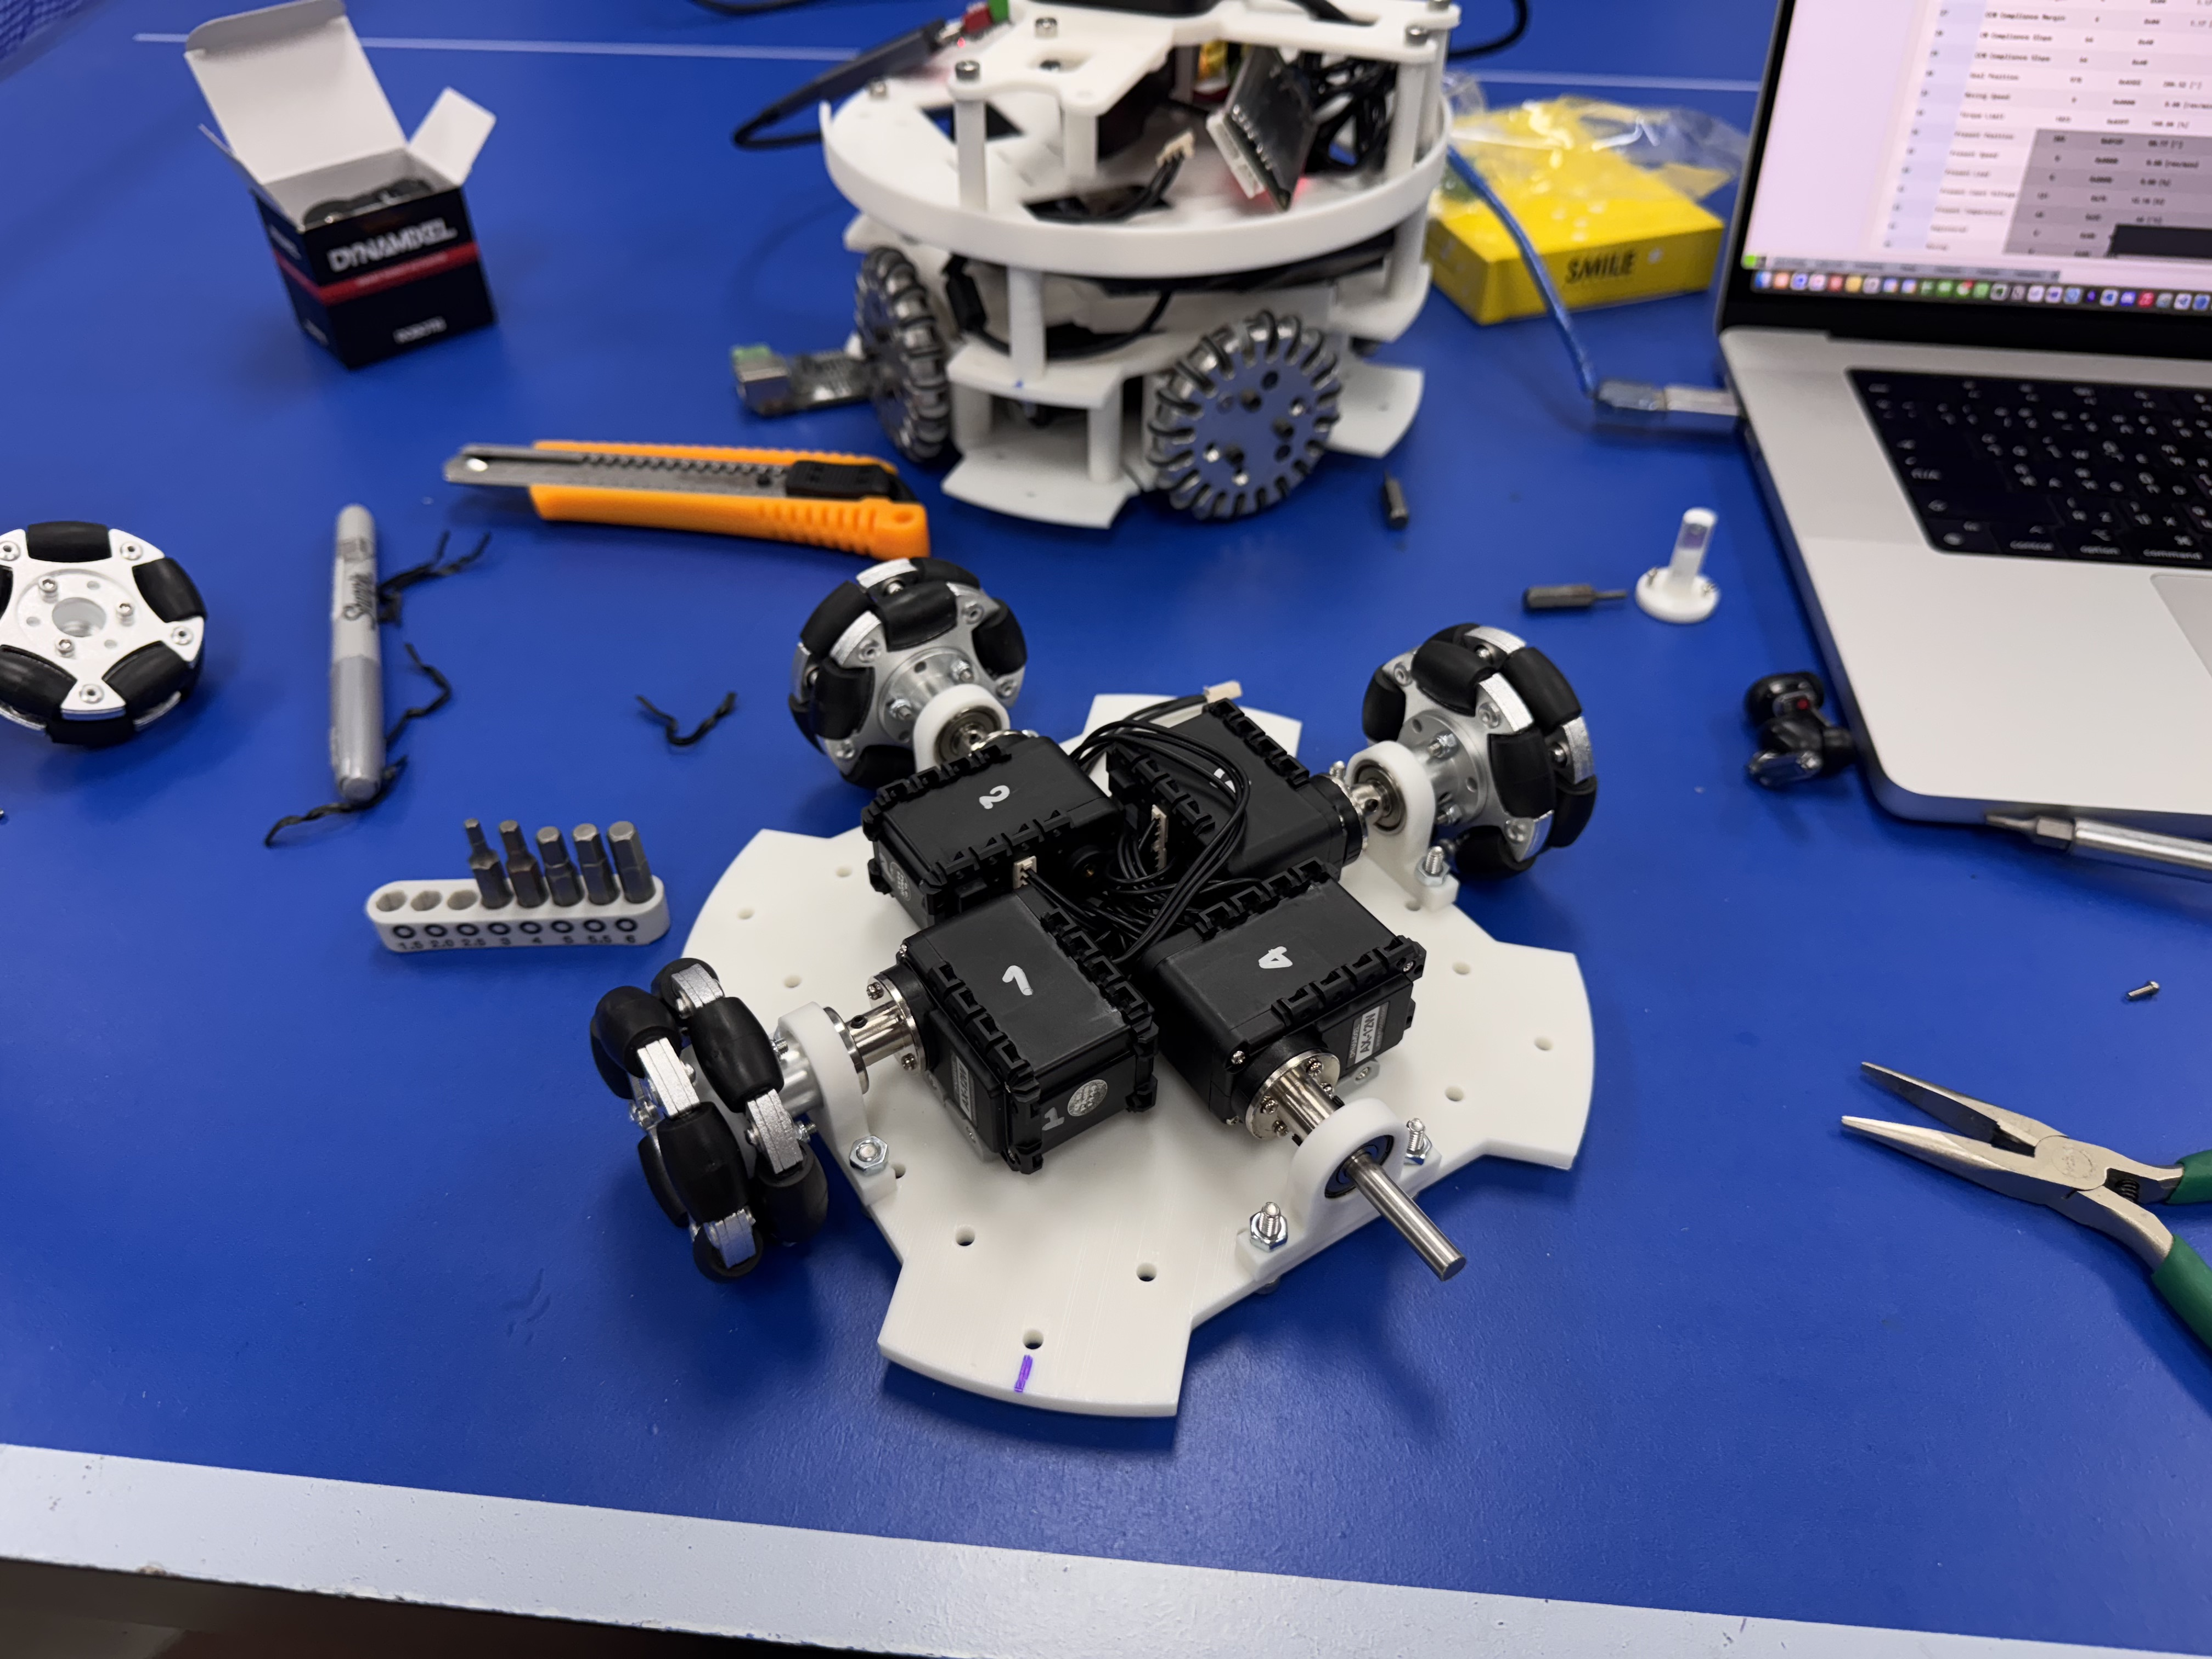
\includegraphics[width=0.3\textwidth]{assets/images/hardware/IMG_8285.jpeg} \\
% \small  \\
The metal shaft in \ref{fig:hdinfo-1}(left) are cut to equal length to be attached to the flange. This change from PLA plastic helped to reduce the wobble using the 3D printed shaft as they are deformed while screwing the lock screw at the wheel flange.

A part added to complete the perception of the robot is the LiDAR and the camera combo for object detection and GraphSLAM. For the mounting of the camera, The camera sensor FOV being directly below the LiDAR is beneficial to reduce parallax error and produce more accurate measurement of an object. For this process, we took apart the Logitech C920 to find where the sensor is location and best match the X, Y error to the already modelled LiDAR Mount. 
The 2 image attached in \ref{fig:camera-mount} are the modeled camera mount and the fitment of the camera to the mount, the designing of the snap fit required accurate measurement of the camera. The tool of choice is an analog vernier caliper. The final printed result is a very tight fit of the camera and the X, Y axis aligned quite well, the result of which are explored in the computer vision section of this report.

\begin{figure} [H]
    \centering
    \begin{tabular}{@{}p{8cm}@{\hspace{0.5cm}}c@{\hspace{0.5cm}}c@{}}
        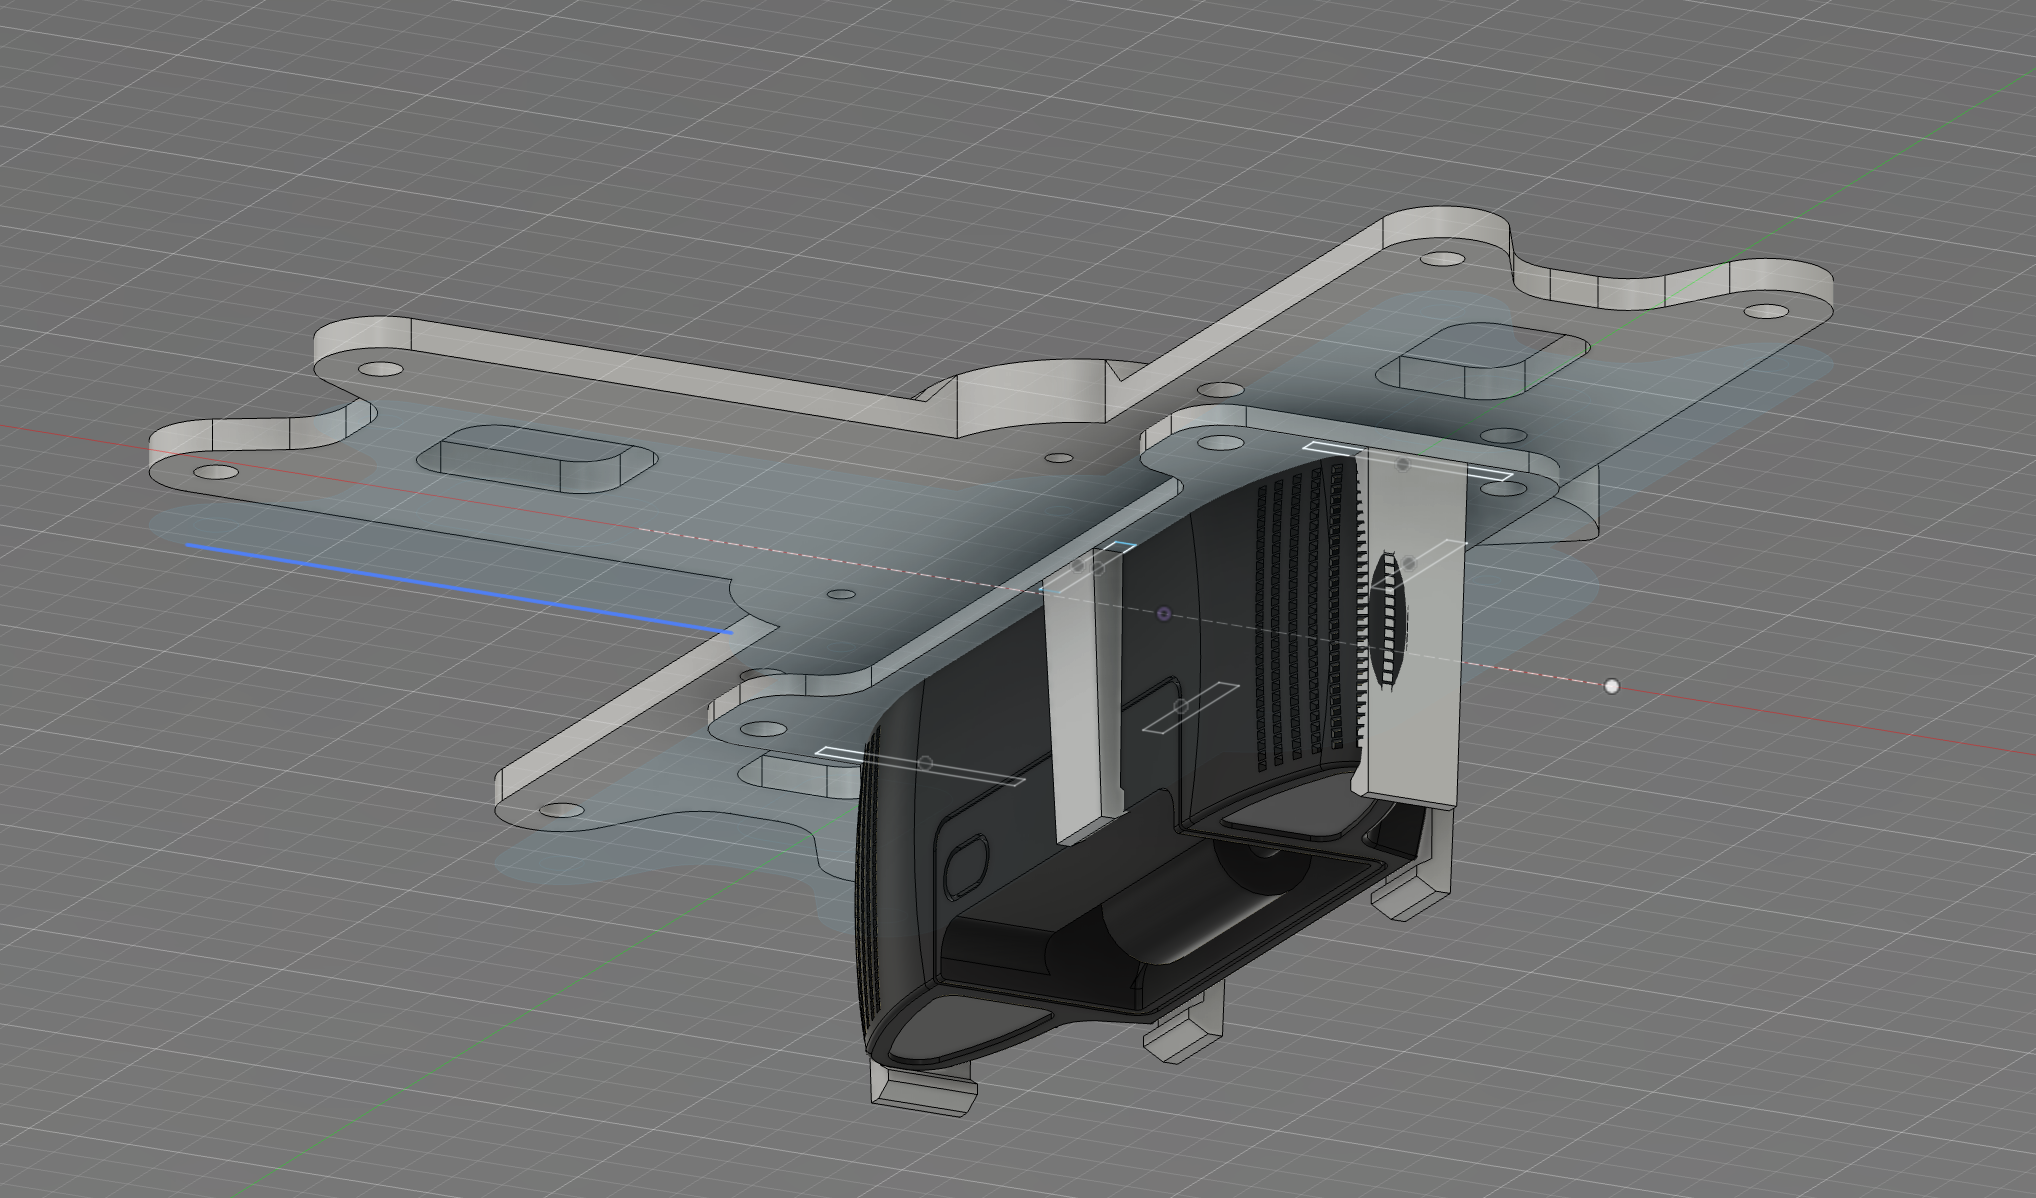
\includegraphics[width=0.5\textwidth]{assets/images/hardware/cad-camera-mount.png} &
        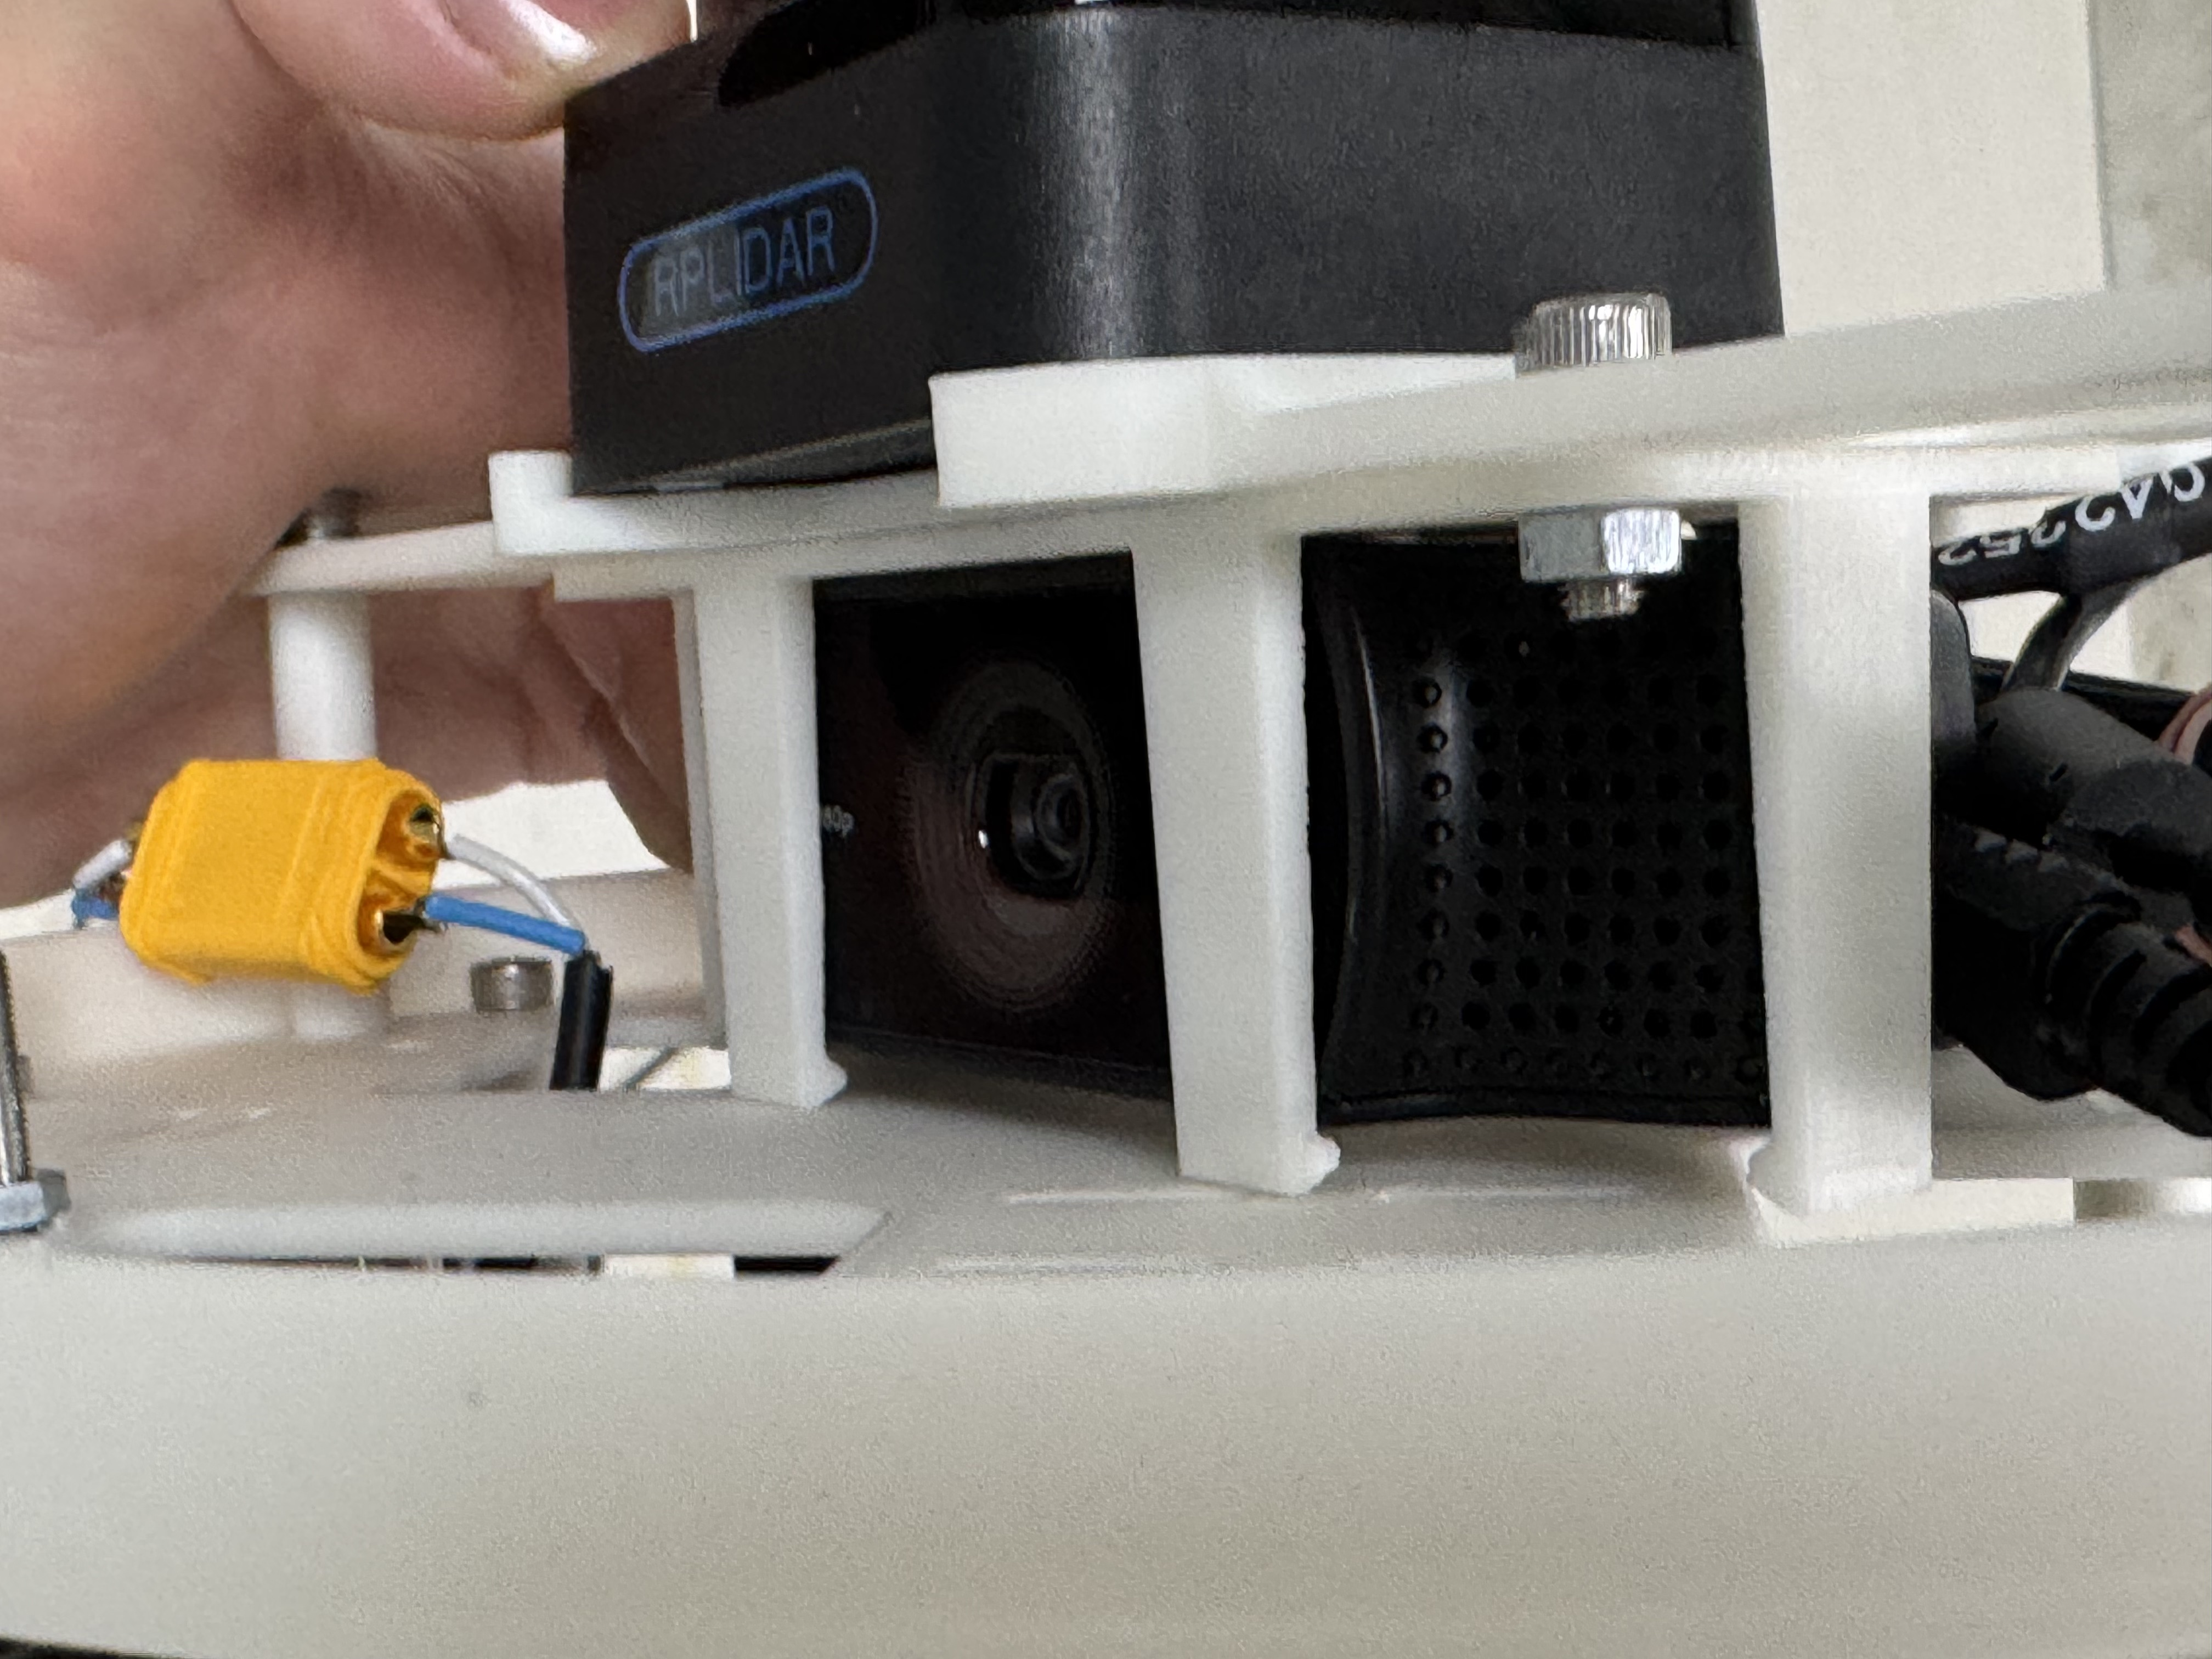
\includegraphics[width=0.5\textwidth]{assets/images/hardware/IMG_9878.jpeg} & \\
        \small Screenshot of a camera mount directly below the LiDAR &
        \small Image of the printed camera mount&
    \end{tabular}
    \caption{Image of the camera mounts }
    \label{fig:camera-mount}
\end{figure}